%% Draft for the Journal of Systems and Software (Elsevier).
%% Compile with the elsarticle class (bundled with TeX Live / Overleaf):
%%   latexmk -pdf main.tex
\documentclass[preprint,12pt]{elsarticle}

\usepackage{amsmath}
\usepackage{booktabs}
\usepackage{graphicx}
\usepackage{xcolor}
\usepackage{listings}
\usepackage{tikz}
\usetikzlibrary{positioning,arrows.meta,fit,backgrounds}
\usepackage[hidelinks]{hyperref}

\newcommand{\todo}[1]{\textcolor{red}{[TODO: #1]}}
\newcommand{\tool}{\textsc{Container Preflight}}
\lstset{basicstyle=\ttfamily\footnotesize,breaklines=true,frame=single,columns=fullflexible}

\journal{Journal of Systems and Software}

\begin{document}

\begin{frontmatter}

\title{Predicting Container Deployment Failures Before Execution by Jointly Analyzing Container Artifacts and Host Environments}

\author[1]{Raphael Gab-Momoh\corref{cor1}}
\ead{rdgabmomoh@gmail.com}
\cortext[cor1]{Corresponding author. ORCID: \href{https://orcid.org/0009-0000-9090-7957}{0009-0000-9090-7957}}
\affiliation[1]{organization={Paynautik Limited},city={Lagos},country={Nigeria}}

\begin{abstract}
Containerized projects that work on one machine routinely fail on another: an image lacks the host's CPU architecture, a Compose file needs more memory than the Docker virtual machine has, a \texttt{COPY} source is excluded by \texttt{.dockerignore}, a port is already taken. Existing tools inspect either the artifacts (Dockerfile linters) or the host (daemon diagnostics), never both, and Docker itself reports only the first failure it reaches. We present \tool{}, an approach and tool that predicts deployment failures before anything runs by joining three views: requirements extracted from Compose files and Dockerfiles with Docker's own parsers, a capability profile of the host (including the virtual machine that Docker Desktop and Colima run on macOS), and image metadata read directly from registries. Checks that depend on facts that cannot be established are grouped under a single root cause through an explicit causal graph, and a learning component turns observed failures into shareable rules that are generalized by later failures and specialized by successful runs. We estimated 95k GitHub issues across 32 failure categories, correcting search counts by verified precision, and labeled two stratified samples. On a held-out sample drawn after the rules were frozen, \tool{} fully predicted 33\% of local Docker failures and at least partially predicted 58\% (58\% weighted by category prevalence); categories it does not target are dominated by runtime behavior such as DNS resolution and health checks. On two real engines (Colima and Docker Desktop) on the same machine, 8 of 11 initial predictions matched the actual failure, 6 word for word, and the same project received different, confirmed predictions per engine. \todo{Inter-rater agreement (Cohen's $\kappa$) on 40 held-out issues.}
\end{abstract}

\begin{keyword}
containers \sep Docker \sep Docker Compose \sep configuration errors \sep failure prediction \sep root cause analysis
\end{keyword}

\end{frontmatter}

%% ---------------------------------------------------------------------
\section{Introduction}
\label{sec:intro}

Containers promised that software runs the same everywhere. In practice a container project is the product of its artifacts \emph{and} the machine it runs on. The same \texttt{compose.yaml} may start on a developer's Intel laptop and fail on a colleague's Apple silicon machine because an image ships only \texttt{linux/amd64}; it may start on Docker Desktop and fail on a Linux server because \texttt{vm.max\_map\_count} is too low for Elasticsearch; it may build on one machine and fail on another that lacks the BuildKit plugin required by \texttt{RUN --mount}.

These failures share three properties that make them costly. First, they are \emph{relational}: neither the artifact nor the host is wrong in isolation. Second, they are \emph{sequential}: Docker stops at the first failure, so a project with five problems is fixed through five failed runs. Third, their error messages point at symptoms: ``Cannot connect to the Docker daemon'' says nothing about the stale context that caused it, and ``exec format error'' says nothing about which image lacks which architecture.

Existing tools address one side. Dockerfile linters such as Hadolint~\cite{hadolint} and research systems such as Binnacle~\cite{henkel2020binnacle} check artifacts against best-practice rules; repair tools such as Shipwright~\cite{henkel2021shipwright} fix broken builds after they fail. Host diagnostics (\texttt{docker info}, Docker Desktop's troubleshooter) report the machine's state without reference to what a project needs. Early detection of configuration errors has been studied for server software~\cite{xu2016pcheck}, but not for the joint space of container artifacts and container hosts.

This paper makes the following contributions:
\begin{enumerate}
  \item \textbf{Joint analysis.} An approach that predicts container build and start-up failures before execution by matching requirements extracted from Compose files, Dockerfiles or \texttt{docker run} commands against a capability profile of the host and image metadata read from registries without pulling (\S\ref{sec:approach}).
  \item \textbf{Root-cause grouping.} A causal fact graph under which a check that needs an unknown fact is reported once under the fact's root cause, including specific diagnoses of why a Docker daemon is unreachable (\S\ref{sec:causal}).
  \item \textbf{Learning from failures.} A rule learner that turns an observed failure into a shareable rule, generalizes it with further failures and specializes it with successful runs (\S\ref{sec:learn}).
  \item \textbf{Evaluation.} A failure taxonomy from 95k verified GitHub issues, a labeled development sample and a held-out test sample, and field validation on two Docker engines (\S\ref{sec:eval}). All data and scripts are released.
\end{enumerate}

%% ---------------------------------------------------------------------
\section{Motivating example}
\label{sec:motivation}

Listing~\ref{lst:shop} shows an excerpt of a Compose project. On an Apple silicon Mac running Colima with default settings, \texttt{docker compose up} fails first with \texttt{error getting credentials} (the Docker configuration still names Docker Desktop's credential helper, which was uninstalled). After fixing that, it fails with \texttt{the --mount option requires BuildKit}. After installing buildx, it fails on a missing \texttt{COPY} source, then on a port clash, then on a missing bind-mounted file, and finally SQL Server crashes under QEMU emulation.

\begin{lstlisting}[caption={Excerpt of the example project.},label={lst:shop}]
services:
  web:
    build: ./web                    # RUN --mount=type=cache ...
    ports: ["8080:80"]
    deploy: {replicas: 2}
    volumes: ["./nginx/nginx.conf:/etc/nginx/nginx.conf:ro"]
  api:
    image: node:20-alpine
    ports: ["8080:3000"]
  db:
    image: mcr.microsoft.com/mssql/server:2022-latest
\end{lstlisting}

\tool{} reports all of these in one run of about four seconds, each with the evidence from both sides and the error Docker would print. On Docker Desktop on the same machine it reports a different set: the credential helper and BuildKit checks pass, and SQL Server is only a warning because Desktop runs amd64 under Rosetta, where it starts successfully (\S\ref{sec:field}).

%% ---------------------------------------------------------------------
\section{Approach}
\label{sec:approach}

\tool{} builds three views and evaluates rules over their join (Figure~\ref{fig:arch}).

\begin{figure}[t]
\centering
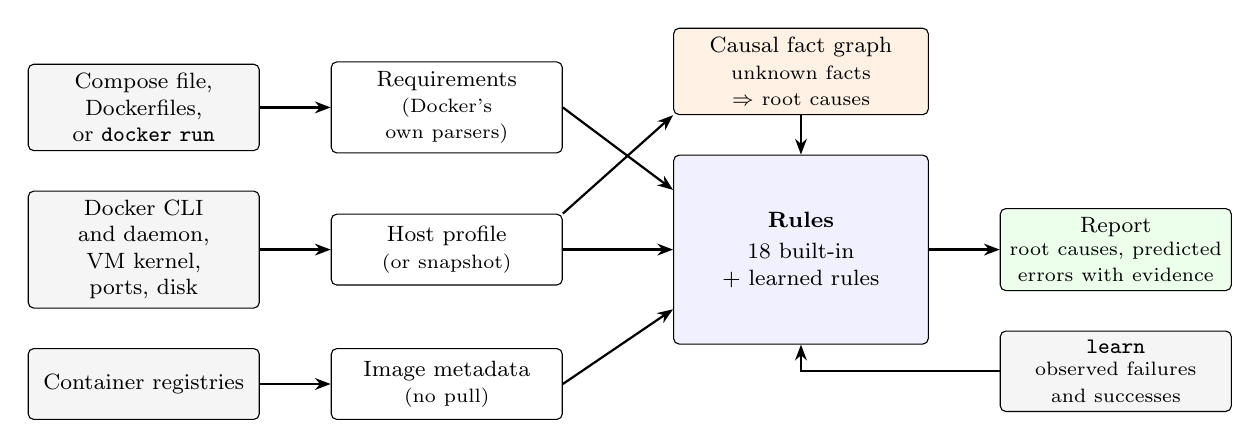
\begin{tikzpicture}[
  font=\footnotesize,
  box/.style={draw, rounded corners=2pt, align=center, minimum height=9mm, text width=27mm, fill=white},
  src/.style={box, fill=gray!8},
  arr/.style={-{Stealth[length=2mm]}, thick},
  node distance=5mm and 9mm]
\node[src] (proj) {Compose file, Dockerfiles,\\ or \texttt{docker run}};
\node[src, below=of proj] (hostsrc) {Docker CLI and daemon,\\ VM kernel, ports, disk};
\node[src, below=of hostsrc] (reg) {Container registries};
\node[box, right=of proj] (req) {Requirements\\ \scriptsize (Docker's own parsers)};
\node[box, right=of hostsrc] (cap) {Host profile\\ \scriptsize (or snapshot)};
\node[box, right=of reg] (meta) {Image metadata\\ \scriptsize (no pull)};
\node[box, right=14mm of cap, text width=30mm, minimum height=24mm, fill=blue!6] (rules) {\textbf{Rules}\\[2pt] 18 built-in\\ + learned rules};
\node[box, above=of rules, text width=30mm, fill=orange!10] (graph) {Causal fact graph\\ \scriptsize unknown facts $\Rightarrow$ root causes};
\node[box, right=of rules, text width=27mm, fill=green!8] (rep) {Report\\ \scriptsize root causes, predicted\\ errors with evidence};
\node[box, below=of rep, text width=27mm, fill=gray!8] (learn) {\texttt{learn}\\ \scriptsize observed failures\\ and successes};
\draw[arr] (proj) -- (req); \draw[arr] (hostsrc) -- (cap); \draw[arr] (reg) -- (meta);
\draw[arr] (req.east) -- (rules.155);
\draw[arr] (cap) -- (rules);
\draw[arr] (meta.east) -- (rules.205);
\draw[arr] (cap.north east) -- (graph.south west);
\draw[arr] (graph) -- (rules);
\draw[arr] (rules) -- (rep);
\draw[arr] (learn.west) -| (rules.south);
\end{tikzpicture}
\caption{Overview. Requirements, host capabilities and registry metadata are extracted independently and joined by rules. Facts that cannot be established become root causes that block dependent rules. \texttt{learn} adds rules from observed runs.}
\label{fig:arch}
\end{figure}

\subsection{Project requirements}
Compose files are loaded with \texttt{compose-go}, the library Docker Compose uses, so interpolation, \texttt{.env} files, profiles and path resolution behave as in Compose. Dockerfiles are parsed with BuildKit's Dockerfile frontend. For each build, \tool{} computes the set of stages BuildKit will actually build for the requested target (following \texttt{FROM}, \texttt{COPY --from} and \texttt{RUN --mount from=} edges), because problems in unreachable stages do not break builds. From these it extracts: images to pull and the platform each will be requested for; base images of reachable stages; memory limits and reservations times replicas; published ports; bind mounts and their options; \texttt{COPY}/\texttt{ADD} sources, resolved against the build context and \texttt{.dockerignore} with BuildKit's pattern matcher; BuildKit-only syntax; Compose features with minimum versions; interpolated variables; GPU requests; and the container user. Raw YAML is walked separately to keep line numbers for every requirement. Commands such as \texttt{docker run} are parsed into the same model.

\subsection{Host capabilities}
The host profile records the daemon's platform, memory, runtimes and security options from \texttt{docker info}; Compose and buildx versions; emulated platforms and the emulation mechanism (QEMU or Rosetta); kernel settings; free disk where images are stored; images already present; ports held by processes and containers; and credential helpers. On macOS the daemon runs in a virtual machine, so memory and kernel settings of the \emph{VM} matter, not the laptop's. \tool{} reads them inside the VM (for Colima, through \texttt{colima ssh}; for Docker Desktop, from the VM's command line, which also reveals the folders actually shared with the VM). Profiles can be saved as \emph{snapshots} and checked against from another machine, so a developer can predict failures on a CI runner or server without access to it.

\subsection{Registry metadata}
For each image to be pulled, \tool{} reads the manifest or manifest list from the registry, recording available platforms, the compressed size for the requested platform, and the configured user. Whether a reference is a single-platform image or a manifest list matters: a list without the host's platform makes \texttt{docker pull} fail, whereas a single foreign-platform image is pulled and needs emulation to run.

\subsection{Rules}
Each rule joins a requirement with a capability and emits a finding with severity, evidence from both sides, a fix, a source location, and the error Docker would print. Table~\ref{tab:rules} lists the 18 built-in rules. A small knowledge base records host requirements invisible in manifests, each tied to the error the image prints (e.g., SQL Server's 2000~MB minimum and its crash under QEMU; Elasticsearch's \texttt{vm.max\_map\_count}, skipped in single-node mode where its bootstrap checks do not apply).

\begin{table}[t]
\centering\footnotesize
\caption{Built-in rules.}
\label{tab:rules}
\begin{tabular}{@{}lp{0.62\linewidth}@{}}
\toprule
Rule & Predicts \\
\midrule
\texttt{image.exists} & tag or repository missing, or private \\
\texttt{image.platform} & no variant for the host platform; emulation unavailable; known crashes under QEMU \\
\texttt{registry.credentials} & configured credential helper not installed \\
\texttt{build.context} & \texttt{COPY}/\texttt{ADD} source missing, excluded by \texttt{.dockerignore}, or outside the context \\
\texttt{build.buildkit} & BuildKit-only syntax with the legacy builder \\
\texttt{compose.version} & Compose features newer than the installed Compose \\
\texttt{compose.env} & unset or required variables \\
\texttt{resources.memory} & known image minimums and total limits vs.\ Docker's memory \\
\texttt{resources.disk} & image size vs.\ free space (VM and host volume) \\
\texttt{host.disk} & too little host space for a VM-based engine \\
\texttt{host.installer} & Docker Desktop running from its installer image \\
\texttt{resources.gpu} & GPU requests without an NVIDIA runtime \\
\texttt{kernel.sysctl} & \texttt{vm.max\_map\_count} below image requirement \\
\texttt{ports.conflict} & services or replicas publishing one host port \\
\texttt{ports.host} & host port held by a process or another project's container; rootless privileged ports \\
\texttt{mounts.bind} & missing bind sources that become directories \\
\texttt{mounts.permissions} & non-root writes to root-owned or foreign-owned binds; SELinux labels \\
\texttt{mounts.sharing} & paths outside Docker Desktop's shared folders \\
\bottomrule
\end{tabular}
\end{table}

%% ---------------------------------------------------------------------
\section{Root-cause grouping}
\label{sec:causal}

Facts form a directed graph: the Docker CLI must exist before the daemon can be queried; the daemon must answer before its platform or memory are known; whether the daemon is \emph{local} is derived from the CLI context, not from the daemon, so port and bind-mount checks still run while the daemon is down. Each rule declares the facts it needs. When a fact cannot be established, the engine walks to the top-most failed ancestor and reports every dependent rule once under that root. Unknown is never reported as pass: when \tool{} cannot read a kernel setting or the emulation mechanism, it emits a warning rather than silently passing, a distinction that the field validation showed to matter (\S\ref{sec:field}).

A daemon that cannot be reached is further diagnosed from local evidence: whether the context's socket exists and which engine owns it, which engines are installed or running, whether commands time out (a starting or memory-starved VM), whether Docker Desktop runs from its installer image, and free host disk. On the author's machine this turned ``Cannot connect to the Docker daemon'' into ``Docker context \texttt{desktop-linux} still points to Docker Desktop, which is not installed'' with the fix \texttt{colima start}, which worked.

%% ---------------------------------------------------------------------
\section{Learning rules from failures}
\label{sec:learn}

Built-in rules cannot anticipate application-specific failures. \texttt{learn} wraps a command (typically \texttt{docker compose up}), and on failure extracts the decisive log line with a keyword-weighted score that down-weights generic wrappers. The line is generalized into a signature by replacing addresses, identifiers, paths and numbers. The service's features at the time (image repository, platform, emulation mechanism, memory bucket, builder, and which environment variables are set, never their values) become the rule's conditions, starting from features that are unusual or plausibly causal.

Rules are refined in the manner of version-space learning~\cite{mitchell1982generalization}. A later failure with the same signature drops conditions the observations disagree on (generalization). A successful run that satisfies every condition adds a feature on which all failures agree and the success differs (specialization); if none exists, the rule is marked unreliable and no longer reported. Rules live in the project repository, so one developer's failure becomes a prediction for everyone.

In a real run, Postgres started without a password failed; \texttt{learn} created a rule conditioned on the image. After a password was added, the successful run specialized the rule to \texttt{env.POSTGRES\_PASSWORD=unset}, and \tool{} then flagged a different project using \texttt{postgres:17} without a password.

%% ---------------------------------------------------------------------
\section{Evaluation}
\label{sec:eval}

We ask:
\textbf{RQ1} How common are the failures \tool{} targets?
\textbf{RQ2} What share of real local Docker failures would \tool{} have predicted?
\textbf{RQ3} Do predictions match reality on real engines?

\subsection{RQ1: Failure landscape}
We defined 32 failure categories by the error text Docker or the image prints, including 7 categories \tool{} does not target, and counted GitHub issues created since 2021 per category. Because issue search matches loosely, we fetched 30 sampled issues per category with their comments and checked for the exact error text, giving a precision estimate and an adjusted count. Precision was at least 0.83 for all but three categories: OOMKilled (0.37, largely Kubernetes), ``network not found'' (0.33) and the SQL Server memory message (0.0). For ``network not found'' the check requires Docker's own phrasing (\texttt{network <name> not found} or \texttt{declared as external, but could not be found}); an earlier, looser check that only required both words had reported 0.97. The labeled samples for this category (8 of 245 issues) were drawn under the looser check.

Of the 95k adjusted issues, 80\% fall in targeted categories; excluding OOMKilled, which is dominated by Kubernetes, 68\%. The largest targeted categories are platform mismatches (11.7k), missing images (10.6k) and port conflicts (5.1k); the largest untargeted are Docker networks not found (6.1k), volume permissions (6.1k, subsequently addressed by \texttt{mounts.permissions}), OCI runtime exec errors (3.5k) and DNS resolution (2.0k). Table~\ref{tab:categories} lists all categories.

\begin{table}[t]
\centering\scriptsize
\caption{Failure categories: GitHub issues since 2021 matching each error, precision of the search (share of 30 sampled issues containing the exact error text), and adjusted estimate. Rule ``--'' marks categories \tool{} does not target; $\dagger$ marks a rule added after mining.}
\label{tab:categories}
\begin{tabular}{@{}llrrr@{}}
\toprule
Category & Rule & Hits & Precision & Adjusted \\
\midrule
memory: OOMKilled & \texttt{resources.memory} & 97,607 & 0.37 & 35,789 \\
network not found & -- & 18,407 & 0.97 & 17,793 \\
image: tag/repo not found & \texttt{image.exists} & 7,405 & 0.93 & 6,911 \\
volume permission denied & \texttt{mounts.permissions}$^\dagger$ & 6,073 & 1.00 & 6,073 \\
platform: exec format error & \texttt{image.platform} & 5,372 & 0.97 & 5,193 \\
address already in use & \texttt{ports.host} & 3,792 & 1.00 & 3,792 \\
image: pull access denied & \texttt{image.exists} & 3,730 & 1.00 & 3,730 \\
platform: requested platform mismatch & \texttt{image.platform} & 3,717 & 1.00 & 3,717 \\
OCI runtime exec failed & -- & 3,479 & 1.00 & 3,479 \\
platform: no matching manifest & \texttt{image.platform} & 2,760 & 1.00 & 2,760 \\
daemon: cannot connect & (root cause) & 2,712 & 1.00 & 2,712 \\
compose: variable not set & \texttt{compose.env} & 2,390 & 0.97 & 2,310 \\
DNS resolution in container & -- & 2,021 & 1.00 & 2,021 \\
build: COPY source not found & \texttt{build.context} & 1,421 & 1.00 & 1,421 \\
emulation: qemu crash & \texttt{image.platform} & 1,301 & 1.00 & 1,301 \\
disk: no space left & \texttt{resources.disk} & 1,241 & 1.00 & 1,241 \\
port already allocated & \texttt{ports.conflict} & 1,239 & 1.00 & 1,239 \\
container healthcheck unhealthy & -- & 1,155 & 1.00 & 1,155 \\
bind: dir onto file & \texttt{mounts.bind} & 707 & 1.00 & 707 \\
bind: source does not exist & \texttt{mounts.bind} & 544 & 1.00 & 544 \\
compose: unsupported property & \texttt{compose.version} & 486 & 1.00 & 486 \\
gpu: no device driver & \texttt{resources.gpu} & 457 & 1.00 & 457 \\
build: BuildKit required & \texttt{build.buildkit} & 443 & 0.97 & 428 \\
build: COPY failed legacy & \texttt{build.context} & 417 & 1.00 & 417 \\
compose: required variable & \texttt{compose.env} & 475 & 0.83 & 396 \\
kernel: vm.max\_map\_count & \texttt{kernel.sysctl} & 369 & 1.00 & 369 \\
credentials helper missing & \texttt{registry.credentials} & 260 & 1.00 & 260 \\
desktop: mounts denied & \texttt{mounts.sharing} & 153 & 1.00 & 153 \\
app config/env missing at runtime & (learned) & 118 & 1.00 & 118 \\
build: outside build context & \texttt{build.context} & 65 & 1.00 & 65 \\
rootless privileged port & \texttt{ports.host} & 39 & 0.87 & 34 \\
memory: mssql minimum & \texttt{resources.memory} & 4,653 & 0.00 & 0 \\
\bottomrule
\end{tabular}
\end{table}


\subsection{RQ2: Predictive coverage}
\paragraph{Protocol} We drew a development sample of 4 verified issues per category (124 issues) and labeled each: whether it is a local Docker failure (not Kubernetes, Podman, application bugs or feature requests), and whether \tool{} would have predicted it before execution given the project files and the host (\emph{yes}), would have addressed its cause only partially (\emph{partial}: a warning where an error resulted, a different input form, a different OS, or only after learning), or not (\emph{no}). We then added rules for misses and froze them (tag \texttt{eval-frozen}). Finally we drew a held-out test sample of 121 issues with a different search ordering, excluding every issue seen before, and labeled it against the frozen rules.

\begin{table}[t]
\centering\footnotesize
\caption{Predictive coverage on local Docker failures.}
\label{tab:coverage}
\begin{tabular}{@{}lrrrrr@{}}
\toprule
Sample & $n$ & Yes & Partial & No & Yes (weighted) \\
\midrule
Development, initial rules & 98 & 42\% & 26\% & 33\% & 31\% \\
Development, after fixes   & 98 & 51\% & 18\% & 31\% & 46\% \\
\textbf{Held-out test}     & \textbf{72} & \textbf{33\%} & \textbf{25\%} & \textbf{42\%} & \textbf{30\%} \\
\bottomrule
\end{tabular}
\end{table}

Table~\ref{tab:coverage} reports results; ``weighted'' reweights categories by their adjusted prevalence. The drop from development to test (51\% to 33\%) shows the development figure was optimistic, as expected for rules written after seeing its misses; the held-out figure is the one we claim. Yes-or-partial remained stable (69\% vs.\ 58\%; 60\% vs.\ 58\% weighted). Misses concentrate on runtime behavior (unhealthy containers, DNS, application errors, OCI exec), which configuration analysis cannot observe.

\paragraph{Agreement} \todo{A second rater, blind to our labels, labeled 40 held-out issues. Report Cohen's $\kappa$~\cite{cohen1960kappa} for scope and for prediction.}

\subsection{RQ3: Field validation}
\label{sec:field}
We ran \tool{} on the example project on an Apple silicon Mac, first with Colima (Ubuntu VM, 1.9~GiB, QEMU, no buildx) and then with Docker Desktop (3.8~GiB VM, Rosetta, buildx), and checked every prediction by executing the corresponding Docker command.

On Colima, 8 of 11 initial predictions identified the real failure, 6 with Docker's exact wording (credential helper, BuildKit, required variable, two port conflicts, bind mount of a missing file) and 2 with different wording, since corrected. One was a false positive: \tool{} predicted that amd64 could not run, but the VM had QEMU registered, which the first version could not see; two were imprecise (a memory prediction masked by an earlier QEMU crash, and a kernel check that passed without data). All three stemmed from facts inside the VM, and reading the VM's kernel fixed them.

On Docker Desktop, the same project received different predictions, each confirmed: SQL Server ran under Rosetta (``ready for client connections'') where it had crashed under QEMU; a bind mount outside the shared folders failed with the predicted \texttt{mounts denied} message. Setting up Docker Desktop also produced a new failure---Desktop launched from its installer image held the socket and hung every command---which \tool{} now diagnoses.

%% ---------------------------------------------------------------------
\section{Discussion and threats to validity}
\label{sec:threats}

\paragraph{Construct} ``Would have predicted'' is a judgment about a counterfactual run; we mitigate it with a written rubric and a blind second rater. Category membership is defined by error text, which excludes failures reported without logs.

\paragraph{Internal} The first author built the tool and labeled both samples. The development sample was used to add rules; we therefore froze rules before drawing the test sample and report the test result. Some predicted error texts and minimum versions were written from documentation and were corrected only where verified.

\paragraph{External} GitHub issues over-represent open-source projects and under-represent failures resolved silently. Field validation covers two engines on one machine; Linux servers, Windows and remote daemons were exercised only through tests and snapshots.

\paragraph{Scope} \tool{} targets configuration and environment mismatches. It does not predict runtime behavior, and learned rules can only predict failures someone has already hit.

%% ---------------------------------------------------------------------
\section{Related work}
\label{sec:related}

\paragraph{Container ``preflight'' tools} Red Hat's \texttt{preflight}~\cite{openshiftpreflight} checks operator bundles and container images against OpenShift certification requirements, and \texttt{kubeadm} runs preflight checks on a machine before creating a Kubernetes cluster. Both validate an artifact or a host against fixed policy; neither predicts whether a given project will build and run on a given host.

\paragraph{Dockerfile analysis and repair} Cito et al.~\cite{cito2017docker} characterized the Docker ecosystem on GitHub and its quality issues. Hadolint~\cite{hadolint} and Binnacle~\cite{henkel2020binnacle} check Dockerfiles against rules; Shipwright~\cite{henkel2021shipwright} repairs broken builds; Wu et al.~\cite{wu2020buildfailures} studied Docker build failures. Recent work repairs Dockerfile drift using project context~\cite{drift2026}. All operate on artifacts; none model the host.

\paragraph{Compose} Ibrahim et al.~\cite{ibrahim2021compose} studied how Docker Compose is used to compose multi-component systems; linters validate Compose syntax. They do not relate files to host capabilities.

\paragraph{Configuration errors} Xu et al.~\cite{xu2016pcheck} detect latent configuration errors early by checking configuration values at initialization. \tool{} applies the early-detection idea across the artifact--host boundary of containers and adds learning from observed failures.

%% ---------------------------------------------------------------------
\section{Conclusion}
\label{sec:conclusion}

Container failures that ``work on my machine'' are relational: they arise between a project and a host. By analyzing both together, grouping unknowns under root causes and learning from observed failures, \tool{} predicted a third of held-out local Docker failures fully and more than half at least partially, before anything ran, and its predictions held up on two real engines. The same join applies to Kubernetes: manifests against a specific cluster's node architectures, allocatable resources, quotas, storage classes, served APIs and admission policies, predicting events such as \texttt{FailedScheduling}, \texttt{ImagePullBackOff} and \texttt{no matches for kind} before deployment, with root-cause grouping and learned rules unchanged. Other future work: runtime-oriented checks such as health checks and container DNS, and a study with developers measuring time to a working setup.

\section*{Data availability}
The tool, rules, mined data, samples, labels and scripts are available at \url{https://github.com/raphgm/container-preflight} \todo{archive with a DOI on Zenodo}.

\bibliographystyle{elsarticle-num}
\bibliography{refs}

\end{document}
